\documentclass[12pt]{article}
\usepackage{amsmath, amssymb, amsthm, enumerate, graphicx}
\usepackage[usenames,dvipsnames]{color}
\usepackage{bm}
\usepackage[colorlinks=true,urlcolor=blue]{hyperref}
\usepackage{geometry}
\geometry{margin=1in}
\usepackage{float}
\usepackage{graphics}
\setlength{\marginparwidth}{2.15cm}
\usepackage{booktabs}
\usepackage{enumitem}
\usepackage{epsfig}
\usepackage{setspace}
\usepackage{parskip}
\usepackage[normalem]{ulem}
\usepackage{tikz}
\usetikzlibrary{positioning, arrows, automata}
\usepackage{pgfplots}
\pgfplotsset{compat=newest}
\usepackage[font=scriptsize]{subcaption}
\usepackage{float}
\usepackage[]{algorithm2e}
\usepackage{environ}
\usepackage{bbm}
\usepackage{graphicx}
\usepackage{titling}
\usepackage{url}
\usepackage{xcolor}
\usepackage{lipsum}
\usepackage{lastpage}
\usepackage[colorlinks=true,urlcolor=blue]{hyperref}
\usepackage{multicol}
\usepackage{tabularx}
\usepackage{comment}
\usepackage[utf8]{inputenc}
\usepackage{amssymb}
\usepackage{setspace}
\usepackage{marvosym}
\usepackage{wrapfig}
\usepackage{datetime}
\usepackage[many]{tcolorbox}
\usepackage{array}
\usepackage{multirow}
\usepackage{wasysym}
\usepackage{cancel}
\usepackage{cprotect}
\usepackage{listings}
\usepackage{color}


\newcommand{\R}{\mathbb{R}}
\newcommand{\blackcircle}{\tikz\draw[black,fill=black] (0,0) circle (1ex);}
\renewcommand{\circle}{\tikz\draw[black] (0,0) circle (1ex);}

\newtcolorbox[]{solution}[1][]{%
    breakable,
    enhanced,
    colback=white,
    title=Solution,
    #1
}

% SOLUTION environment
\NewEnviron{soln}{
\leavevmode\color{red}\ignorespaces \textbf{Solution} \BODY }{}

% QUESTION AUTHORS environment
\NewEnviron{qauthor}{
\leavevmode\color{blue}\ignorespaces \textbf{Author} \BODY}{}

% SOLUTION environment
\NewEnviron{qlearningobjective}{
\leavevmode\color{blue}\ignorespaces \textbf{Learning Objective } \BODY }{}

% TO ONLY SHOW HOMEWORK QUESTIONS, include following (else comment out):
% \RenewEnviron{soln}{}
 \RenewEnviron{qauthor}{}
 \RenewEnviron{qlearningobjective}{}


%\newcommand{\norm}[1]{\lVert #1 \rVert}
%\newcommand{\st}{\mathrm{s.t.}}

\makeatletter
\newcommand{\removelatexerror}{\let\@latex@error\@gobble}
\makeatother

\newcommand{\argmax}{\mathop{\mathrm{argmax}}}
\newcommand{\argmin}{\mathop{\mathrm{argmin}}}

%%%%%%%%%%%%%%%%%%%%%%%%%%%%%%%%%%%%%%%%%%%
% Custom Math                             %
%%%%%%%%%%%%%%%%%%%%%%%%%%%%%%%%%%%%%%%%%%%


%%%%%%%%%%%%%%%%%%%%%%%%%%%%%%%%%%%%%%%%%%
% Custom commands                        %
%%%%%%%%%%%%%%%%%%%%%%%%%%%%%%%%%%%%%%%%%%

\newcommand{\vc}[1]{\boldsymbol{#1}}
\newcommand{\adj}[1]{\frac{d J}{d #1}}
\newcommand{\chain}[2]{\adj{#2} = \adj{#1}\frac{d #1}{d #2}}

% mathcal
\newcommand{\Ac}{\mathcal{A}}
\newcommand{\Bc}{\mathcal{B}}
\newcommand{\Cc}{\mathcal{C}}
\newcommand{\Dc}{\mathcal{D}}
\newcommand{\Ec}{\mathcal{E}}
\newcommand{\Fc}{\mathcal{F}}
\newcommand{\Gc}{\mathcal{G}}
\newcommand{\Hc}{\mathcal{H}}
\newcommand{\Ic}{\mathcal{I}}
\newcommand{\Jc}{\mathcal{J}}
\newcommand{\Kc}{\mathcal{K}}
\newcommand{\Lc}{\mathcal{L}}
\newcommand{\Mc}{\mathcal{M}}
\newcommand{\Nc}{\mathcal{N}}
\newcommand{\Oc}{\mathcal{O}}
\newcommand{\Pc}{\mathcal{P}}
\newcommand{\Qc}{\mathcal{Q}}
\newcommand{\Rc}{\mathcal{R}}
\newcommand{\Sc}{\mathcal{S}}
\newcommand{\Tc}{\mathcal{T}}
\newcommand{\Uc}{\mathcal{U}}
\newcommand{\Vc}{\mathcal{V}}
\newcommand{\Wc}{\mathcal{W}}
\newcommand{\Xc}{\mathcal{X}}
\newcommand{\Yc}{\mathcal{Y}}
\newcommand{\Zc}{\mathcal{Z}}

% mathbb
\newcommand{\Ab}{\mathbb{A}}
\newcommand{\Bb}{\mathbb{B}}
\newcommand{\Cb}{\mathbb{C}}
\newcommand{\Db}{\mathbb{D}}
\newcommand{\Eb}{\mathbb{E}}
\newcommand{\Fb}{\mathbb{F}}
\newcommand{\Gb}{\mathbb{G}}
\newcommand{\Hb}{\mathbb{H}}
\newcommand{\Ib}{\mathbb{I}}
\newcommand{\Jb}{\mathbb{J}}
\newcommand{\Kb}{\mathbb{K}}
\newcommand{\Lb}{\mathbb{L}}
\newcommand{\Mb}{\mathbb{M}}
\newcommand{\Nb}{\mathbb{N}}
\newcommand{\Ob}{\mathbb{O}}
\newcommand{\Pb}{\mathbb{P}}
\newcommand{\Qb}{\mathbb{Q}}
\newcommand{\Rb}{\mathbb{R}}
\newcommand{\Sb}{\mathbb{S}}
\newcommand{\Tb}{\mathbb{T}}
\newcommand{\Ub}{\mathbb{U}}
\newcommand{\Vb}{\mathbb{V}}
\newcommand{\Wb}{\mathbb{W}}
\newcommand{\Xb}{\mathbb{X}}
\newcommand{\Yb}{\mathbb{Y}}
\newcommand{\Zb}{\mathbb{Z}}

% mathbf lowercase
\newcommand{\av}{\mathbf{a}}
\newcommand{\bv}{\mathbf{b}}
\newcommand{\cv}{\mathbf{c}}
\newcommand{\dv}{\mathbf{d}}
\newcommand{\ev}{\mathbf{e}}
\newcommand{\fv}{\mathbf{f}}
\newcommand{\gv}{\mathbf{g}}
\newcommand{\hv}{\mathbf{h}}
\newcommand{\iv}{\mathbf{i}}
\newcommand{\jv}{\mathbf{j}}
\newcommand{\kv}{\mathbf{k}}
\newcommand{\lv}{\mathbf{l}}
\newcommand{\mv}{\mathbf{m}}
\newcommand{\nv}{\mathbf{n}}
\newcommand{\ov}{\mathbf{o}}
\newcommand{\pv}{\mathbf{p}}
\newcommand{\qv}{\mathbf{q}}
\newcommand{\rv}{\mathbf{r}}
\newcommand{\sv}{\mathbf{s}}
\newcommand{\tv}{\mathbf{t}}
\newcommand{\uv}{\mathbf{u}}
\newcommand{\vv}{\mathbf{v}}
\newcommand{\wv}{\mathbf{w}}
\newcommand{\xv}{\mathbf{x}}
\newcommand{\yv}{\mathbf{y}}
\newcommand{\zv}{\mathbf{z}}

% mathbf uppercase
\newcommand{\Av}{\mathbf{A}}
\newcommand{\Bv}{\mathbf{B}}
\newcommand{\Cv}{\mathbf{C}}
\newcommand{\Dv}{\mathbf{D}}
\newcommand{\Ev}{\mathbf{E}}
\newcommand{\Fv}{\mathbf{F}}
\newcommand{\Gv}{\mathbf{G}}
\newcommand{\Hv}{\mathbf{H}}
\newcommand{\Iv}{\mathbf{I}}
\newcommand{\Jv}{\mathbf{J}}
\newcommand{\Kv}{\mathbf{K}}
\newcommand{\Lv}{\mathbf{L}}
\newcommand{\Mv}{\mathbf{M}}
\newcommand{\Nv}{\mathbf{N}}
\newcommand{\Ov}{\mathbf{O}}
\newcommand{\Pv}{\mathbf{P}}
\newcommand{\Qv}{\mathbf{Q}}
\newcommand{\Rv}{\mathbf{R}}
\newcommand{\Sv}{\mathbf{S}}
\newcommand{\Tv}{\mathbf{T}}
\newcommand{\Uv}{\mathbf{U}}
\newcommand{\Vv}{\mathbf{V}}
\newcommand{\Wv}{\mathbf{W}}
\newcommand{\Xv}{\mathbf{X}}
\newcommand{\Yv}{\mathbf{Y}}
\newcommand{\Zv}{\mathbf{Z}}

% bold greek lowercase
\newcommand{\alphav     }{\boldsymbol \alpha     }
\newcommand{\betav      }{\boldsymbol \beta      }
\newcommand{\gammav     }{\boldsymbol \gamma     }
\newcommand{\deltav     }{\boldsymbol \delta     }
\newcommand{\epsilonv   }{\boldsymbol \epsilon   }
\newcommand{\varepsilonv}{\boldsymbol \varepsilon}
\newcommand{\zetav      }{\boldsymbol \zeta      }
\newcommand{\etav       }{\boldsymbol \eta       }
\newcommand{\thetav     }{\boldsymbol \theta     }
\newcommand{\varthetav  }{\boldsymbol \vartheta  }
\newcommand{\iotav      }{\boldsymbol \iota      }
\newcommand{\kappav     }{\boldsymbol \kappa     }
\newcommand{\varkappav  }{\boldsymbol \varkappa  }
\newcommand{\lambdav    }{\boldsymbol \lambda    }
\newcommand{\muv        }{\boldsymbol \mu        }
\newcommand{\nuv        }{\boldsymbol \nu        }
\newcommand{\xiv        }{\boldsymbol \xi        }
\newcommand{\omicronv   }{\boldsymbol \omicron   }
\newcommand{\piv        }{\boldsymbol \pi        }
\newcommand{\varpiv     }{\boldsymbol \varpi     }
\newcommand{\rhov       }{\boldsymbol \rho       }
\newcommand{\varrhov    }{\boldsymbol \varrho    }
\newcommand{\sigmav     }{\boldsymbol \sigma     }
\newcommand{\varsigmav  }{\boldsymbol \varsigma  }
\newcommand{\tauv       }{\boldsymbol \tau       }
\newcommand{\upsilonv   }{\boldsymbol \upsilon   }
\newcommand{\phiv       }{\boldsymbol \phi       }
\newcommand{\varphiv    }{\boldsymbol \varphi    }
\newcommand{\chiv       }{\boldsymbol \chi       }
\newcommand{\psiv       }{\boldsymbol \psi       }
\newcommand{\omegav     }{\boldsymbol \omega     }

% bold greek uppercase
\newcommand{\Gammav     }{\boldsymbol \Gamma     }
\newcommand{\Deltav     }{\boldsymbol \Delta     }
\newcommand{\Thetav     }{\boldsymbol \Theta     }
\newcommand{\Lambdav    }{\boldsymbol \Lambda    }
\newcommand{\Xiv        }{\boldsymbol \Xi        }
\newcommand{\Piv        }{\boldsymbol \Pi        }
\newcommand{\Sigmav     }{\boldsymbol \Sigma     }
\newcommand{\Upsilonv   }{\boldsymbol \Upsilon   }
\newcommand{\Phiv       }{\boldsymbol \Phi       }
\newcommand{\Psiv       }{\boldsymbol \Psi       }
\newcommand{\Omegav     }{\boldsymbol \Omega     }



%%%%%%%%%%%%%%%%%%%%%%%%%%%%%%%%%%%%%%%%%%%
% Custom box for highlights               %
%%%%%%%%%%%%%%%%%%%%%%%%%%%%%%%%%%%%%%%%%%%

% Define box and box title style
\tikzstyle{mybox} = [fill=blue!10, very thick,
    rectangle, rounded corners, inner sep=1em, inner ysep=1em]

% \newcommand{\notebox}[1]{
% \begin{tikzpicture}
% \node [mybox] (box){%
%     \begin{minipage}{\textwidth}
%     #1
%     \end{minipage}
% };
% \end{tikzpicture}%
% }

\NewEnviron{notebox}{

\begin{tikzpicture}
\node [mybox] (box){
    \begin{minipage}{\textwidth}
        \BODY
    \end{minipage}
};
\end{tikzpicture}
}


\begin{document}
\section*{}
\begin{center}
  \centerline{\textsc{\LARGE  Homework 6}}
  \vspace{0.5em}
  \centerline{\textsc{\LARGE Learning Theory and Generative Models}\footnote{Compiled on \today{} at \currenttime{}}}
  \vspace{1em}
  \textsc{\large CMU 10-601: Machine Learning (Fall 2018)} \\
  \vspace{0.5em}
  \url{piazza.com/cmu/fall2018/10601bd} \\
  \vspace{0.5em}
  \centerline{OUT: Thursday, Nov 1st, 2018}
  %\today{} at \currenttime{}}}
  \vspace{0.5em}
  \centerline{DUE: Wednesday, Nov 7th, 2018, 11:59pm}
    \centerline{TAs: Brynn Edmunds, Zhuoran Liu, Emilio Arroyo-Fang, George Xu}
\end{center}


\section*{START HERE: Instructions}

\begin{notebox}
Homework 6 covers topics on learning theory, MLE/MAP, and Naive Bayes. The homework includes multiple choice, True/False, and short answer questions. 
\end{notebox}

\begin{itemize}
\item \textbf{Collaboration policy:} Collaboration on solving the homework is allowed, after you have thought about the problems on your own. It is also OK to get clarification (but not solutions) from books or online resources, again after you have thought about the problems on your own. There are two requirements: first, cite your collaborators fully and completely (e.g., ``Jane explained to me what is asked in Question 2.1''). Second, write your solution {\em independently}: close the book and all of your notes, and send collaborators out of the room, so that the solution comes from you only.  See the Academic Integrity Section on the course site for more information: \url{http://www.cs.cmu.edu/~mgormley/courses/10601bd-f18/about.html#7-academic-integrity-policies}

\item\textbf{Late Submission Policy:} See the late submission policy here: \url{http://www.cs.cmu.edu/~mgormley/courses/10601bd-f18/about.html#6-general-policies}

\item\textbf{Submitting your work:} 

\begin{itemize}

\item \textbf{Gradescope:} For written problems such as short answer, multiple choice, derivations, proofs, or plots, we will be using Gradescope (\url{https://gradescope.com/}). Please use the provided template. Submissions can be handwritten onto the template, but should be labeled and clearly legible. If your writing is not legible, you will not be awarded marks. Alternatively, submissions can be written in LaTeX. Regrade requests can be made, however this gives the TA the opportunity to regrade your entire paper, meaning if additional mistakes are found then points will be deducted.
Each derivation/proof should be completed on a separate page. For short answer questions, you \textbf{should not} include your work in your solution.  If you include your work in your solutions, your assignment may not be graded correctly by our AI assisted grader. In addition, please tag the problems to the corresponding pages when submitting your work.

\end{itemize}

% \item \textbf{Materials:} Download from autolab the tar file (``Download handout"). The tar file will contain all the data that you will need in order to complete this assignment.

\end{itemize}

For multiple choice or select all that apply questions, shade in the box or circle in the template document corresponding to the correct answer(s) for each of the questions. For \LaTeX users, use $\blacksquare$ and \blackcircle  for shaded boxes and circles, and don't change anything else.

\clearpage

\section*{Instructions for Specific Problem Types}

For ``Select One" questions, please fill in the appropriate bubble completely:

\begin{quote}
\textbf{Select One:} Who taught this course?
\begin{list}{}
     \item\CIRCLE{} Matt Gormley
     \item\Circle{} Marie Curie
     \item\Circle{} Noam Chomsky
\end{list}
\end{quote}

If you need to change your answer, you may cross out the previous answer and bubble in the new answer:

\begin{quote}
\textbf{Select One:} Who taught this course?
\begin{list}{}
     \item\CIRCLE{} Matt Gormley
     \item\Circle{} Marie Curie\\
     \xcancel{\CIRCLE}{} Noam Chomsky
\end{list}
\end{quote}


For ``Select all that apply" questions, please fill in all appropriate squares completely:

\begin{quote}
\textbf{Select all that apply:} Which are scientists?
    \begin{list}{}
    \item $\blacksquare$ Stephen Hawking 
    \item $\blacksquare$ Albert Einstein
    \item $\blacksquare$ Isaac Newton
    \item $\square$ I don't know
\end{list}
\end{quote}

Again, if you need to change your answer, you may cross out the previous answer(s) and bubble in the new answer(s):

\begin{quote}
\textbf{Select all that apply:} Which are scientists?
    \begin{list}{}
    \item $\blacksquare$ Stephen Hawking 
    \item $\blacksquare$ Albert Einstein
    \item $\blacksquare$ Isaac Newton\\
    \xcancel{$\blacksquare$} I don't know
\end{list}
\end{quote}

For questions where you must fill in a blank, please make sure your final answer is fully included in the given space. You may cross out answers or parts of answers, but the final answer must still be within the given space.

\begin{quote}
\textbf{Fill in the blank:} What is the course number?

\begin{tcolorbox}[fit,height=1cm, width=4cm, blank, borderline={1pt}{-2pt},nobeforeafter]
    \begin{center}\huge10-601\end{center}
    \end{tcolorbox}\hspace{2cm}
    \begin{tcolorbox}[fit,height=1cm, width=4cm, blank, borderline={1pt}{-2pt},nobeforeafter]
    \begin{center}\huge10-\xcancel{7}601\end{center}
    \end{tcolorbox}
\end{quote}

\clearpage


\section{Learning Theory [22 pts]}
\begin{enumerate}
    \item \textbf{[3 pt]} Let $\delta=|H|e^{-\epsilon m}$. According to the PAC theorems discussed in class, which of the following is correct? Select one.

    \textbf{Select one:}
    \begin{list}{}
        \item $\circle$ With probability at least $1- \delta$, every hypothesis with training error at most $\epsilon$ has true error 0.
        \item $\circle$ With probability at least $1-\epsilon$, a random hypothesis with training error 0 has true error at most $\delta$.
        \item $\CIRCLE$ With probability at least $1-\delta$, every hypothesis with training error 0 has true error at most $\epsilon$.
        \item $\circle$ With probability at least $1-\epsilon$, a random hypothesis with true error 0 has training error at most $\delta$.
    \end{list}
    
    
    \item \textbf{[3 pt]} Consider a decision tree learner applied to data where each example is described by 10 boolean variables $X_1, X_2, \cdots, X_{10}$. What is the VC dimension of the hypothesis space used by this decision tree learner?
    
    \textbf{Fill in the blank:}
    
    \begin{tcolorbox}[fit,height=1cm, width=4cm, blank, borderline={1pt}{-2pt},nobeforeafter]
    
    \begin{center}\huge$2^{10}$\end{center}
    \end{tcolorbox}   
    
    
    \item \textbf{[4 pt]} Consider instance space X which is the set of real numbers. What is the VC dimension of hypothesis class $H$, where each hypothesis $h$ in $H$ is of the form  ``if a $<$ x $<$ b or c $<$ x $<$ d then y = 1; otherwise y = 0"?  (i.e., H is an infinite hypothesis class where a, b, c, and d are arbitrary real numbers.

    \textbf{Select one:}
    \begin{list}{}
        \item $\circle$ 2
        \item $\circle$ 3
        \item $\CIRCLE$ 4
        \item $\circle$ 5
        \item $\circle$ 6
    \end{list}
    

    \clearpage
    
    \item \textbf{[3 pt]} Alex is given a classification task to solve. He has no idea where to start, so he decided to try out a decision tree learner with 2 binary features $X_1$ and $X_2$. He recently learned about PAC learning, and would like to know what is the minimum number (N) of data points that would suffice for the PAC criterion with $\epsilon = 0.1$ and $\delta = 0.01$. 
    
    Notice that a valid decision tree may or may not be full, meaning it doesn't have to split on all features.
    
    \textbf{Fill in the blank:}
    
    \begin{tcolorbox}[fit,height=1cm, width=4cm, blank, borderline={1pt}{-2pt},nobeforeafter]
    
    \begin{center}\huge404\end{center}
    \end{tcolorbox} 
    
    
    
    \item \textbf{[3 pt]} Sally thinks Alex shouldn't have used a decision tree with 2 binary features. Instead, she thinks it would be best to use logistic regression with 16 real-valued features in addition to a bias term. Sally overherd Alex talking about this cool concept called PAC learning and she too would like to use it to analyze her method. She first trains her logistic regression model on $N$ examples to obtain a training error $\hat R$. What is the the upper bound on the true error $R$ in terms of $\hat R$, $\delta$, and $N$. You may use big-$\mathcal{O}$ notation.
    
    \textbf{Fill in the blank:}
    
    \begin{tcolorbox}[fit,height=1cm, width=15cm, blank, borderline={1pt}{-2pt},nobeforeafter]
    
    \begin{center}$R \le \hat R + O(\sqrt{\frac{1}{N}\left[17 + ln(\frac{1}{\delta})\right]})$\end{center}
    \end{tcolorbox} 
    
    
    \item \textbf{[3 pt]} Sally wants to argue her method has lower bound on the true error. Assuming Sally has obtained enough data points to satisfy PAC criterion with $\epsilon = 0.1$ and $\delta = 0.01$. Which of the following is true?
    
    \textbf{Select one:}
    \begin{list}{}
        \item $\circle$ Sally is wrong. Alex's method will always classify unseen data more accurately since it is simpler as it only needs 2 binary features.
        \item $\circle$ She must first regularize her model by removing 14 features to make any comparison at all.
        \item $\circle$ It is sufficient to show that the VC Dimension of her classifier is higher than Alex's, therefore having lower bound for the true error.
        \item $\CIRCLE$ It is necessary to show that the training error she achieves is lower than the training error Alex achieves.
    \end{list}
    
    
    \clearpage
    
    \item \textbf{[3 pt]} Write an English description of VC Dimension.

    \begin{tcolorbox}[fit,height=5cm, width=15cm, blank, borderline={1pt}{-2pt},nobeforeafter]
    The $VC-dimension$ of a hypothesis space $H$ is the cardinality of the largest set $S$ that can be shattered by $H$. (A set of points $S$ is shattered by $H$ is there are hypotheses in $H$ that split $S$ in all of the $2^{|S|}$ possible ways)
    \end{tcolorbox}
    
    
\end{enumerate}

\clearpage

\section{MLE/MAP [34 pts]}
\begin{enumerate}

    \item \textbf{[3 pt]} \textbf{True or False:} Suppose you place a Beta prior over the Bernoulli distribution, and attempt to learn the parameter of the Bernoulli distribution from data. Further suppose an adversary chooses ``bad", but finite hyperparameters for your Beta prior in order to confuse your learning algorithm. As the number of training examples grows to infinity, the MAP estimate of $\theta$ can still converge to the MLE estimate of $\theta$.
    
    \textbf{Select One:}
    
    \begin{list}{}
        \item $\CIRCLE$ True
        \item $\circle$ False
    \end{list}
    
    
    \item \textbf{[3 pt]} Let $\theta$ be a random variable with the following probability density function (pdf): 
    \begin{align*}
        f(\theta) &= 
        \begin{cases}
        2\theta  & \text{if } 0 \leq \theta \leq 1 \\
        0  & \text{otherwise}
        \end{cases}
    \end{align*}
    
    Suppose another random variable Y, which is conditioning on $\theta$, follows an exponential distribution with  $\lambda=3\theta$. Recall that the exponential distribution with parameter $\lambda$ has the following pdf:
    
    %$f(y)=\lambda e^{-\lambda y}$ if $y\geq 0$, otherwise $f(y)=0$
    
    \begin{align*}
        f_{exp}(y) &= 
        \begin{cases}
        \lambda e^{-\lambda y}  & \text{if } y\geq 0 \\
        0  & \text{otherwise}
        \end{cases}
    \end{align*}
    
    What is the MAP estimate of $\theta$ given $Y=\frac{2}{3}$ is observed?

    \textbf{Select one:}
    \begin{list}{}
        \item $\circle$ 0
        \item $\circle$ 1/3
        \item $\CIRCLE$ 1
        \item $\circle$ 2
    \end{list}
    
    
    \clearpage
    
    \item \textbf{[3 pt]} In HW3, you have derived the closed form solution for linear regression. Now, we are coming back to linear regression, viewing it as a statistical model, and deriving the MLE and MAP estimate of the parameters in the following questions. 
    
    Assume we have data $D = \{\mathbf{x}^{(i)}, y^{(i)}\}_{i=1}^{N}$, where $\mathbf{x}^{(i)} = (x_1^{(i)}, \cdots, x_M^{(i)})$ . So our data has $N$  instances and each instance has $M$  attributes/features. Each $y^{(i)}$ is generated given $\mathbf{x}^{(i)}$ with additive noise $\epsilon^{(i)} \sim N(0, \sigma^2)$, that is $y^{(i)} = \mathbf{w}^T \mathbf{x}^{(i)} + \epsilon^{(i)}$ where $\mathbf{w}$  is the parameter vector of linear regression. Given this assumption, what is the distribution of y? 

    \textbf{Select one:}
    \begin{list}{}
        \item $\CIRCLE$ $y^{(i)} \sim N(\mathbf{w}^T \mathbf{x}^{(i)}, \sigma^2)$
        \item $\circle$ $y^{(i)} \sim N(0, \sigma^2)$
        \item $\circle$ $y^{(i)} \sim \textit{Uniform}(\mathbf{w}^T \mathbf{x}^{(i)} - \sigma,  \mathbf{w}^T \mathbf{x}^{(i)} + \sigma)$
        \item $\circle$ None of the above
    \end{list}
    
    
    \item \textbf{[4 pt]} The next step is to learn the MLE of the parameters of the linear regression model. Which expression below is the correct conditional log likelihood $\ell(\mathbf{w})$ with the given data?

    \textbf{Select one:}
    \begin{list}{}
        \item $\CIRCLE$ $\sum_{i=1}^{N} [-\log (\sqrt{2\pi\sigma^2}) - \frac{1}{2\sigma^2} (y^{(i)} - \mathbf{w}^T\mathbf{x}^{(i)})^2]$
        \item $\circle$ $\sum_{i=1}^{N} [\log (\sqrt{2\pi\sigma^2}) + \frac{1}{2\sigma^2} (y^{(i)} - \mathbf{w}^T\mathbf{x}^{(i)})^2]$
        \item $\circle$ $\sum_{i=1}^{N} [-\log(\sqrt{2\pi\sigma^2)} - \frac{1}{2\sigma^2} (y^{(i)} - \mathbf{w}^T\mathbf{x}^{(i)})]$
        \item $\circle$ $-\log (\sqrt{2\pi\sigma^2}) + \sum_{i=1}^{N} [-\frac{1}{2\sigma^2} (y^{(i)} - \mathbf{w}^T\mathbf{x}^{(i)})^2]$
    \end{list}
    
    
    \item \textbf{[4 pt]} Then, the MLE of the parameters is just  $\argmax_{\mathbf{w}} \ell(\mathbf{w})$ . Among the following expressions, select ALL that can yield the correct MLE. 

    \textbf{Select all that apply:}
    \begin{list}{}
        \item $\square$ $\argmax_{\mathbf{w}} \sum_{i=1}^{N} [-\log (\sqrt{2\pi\sigma^2}) - \frac{1}{2\sigma^2} (y^{(i)} - \mathbf{w}^T\mathbf{x}^{(i)})]$
        \item $\blacksquare$ $\argmax_{\mathbf{w}} \sum_{i=1}^{N} [-\log (\sqrt{2\pi\sigma^2}) - \frac{1}{2\sigma^2} (y^{(i)} - \mathbf{w}^T\mathbf{x}^{(i)})^2]$
        \item $\blacksquare$ $\argmax_{\mathbf{w}} \sum_{i=1}^{N} [- \frac{1}{2\sigma^2} (y^{(i)} - \mathbf{w}^T\mathbf{x}^{(i)})^2]$
        \item $\square$ $\argmax_{\mathbf{w}} \sum_{i=1}^{N} [- \frac{1}{2} (y^{(i)} - \mathbf{w}^T\mathbf{x}^{(i)})]$
        \item $\blacksquare$ $\argmax_{\mathbf{w}} \sum_{i=1}^{N} [- \frac{1}{2} (y^{(i)} - \mathbf{w}^T\mathbf{x}^{(i)})^2]$
    \end{list}
    
    
    \clearpage
    
    \item \textbf{[3 pt]} According to the above derivations, is the MLE for the conditional log likelihood equivalent to minimizing mean squared errors (MSE) for the linear regression model when making predictions? Why or why not? 

    \textbf{Select one:}
    \begin{list}{}
        \item $\circle$ Yes, because the derivative of the negative conditional log-likelihood has the same form as the derivative of the MSE loss. 
        \item $\CIRCLE$ Yes, because the parameters that maximize the conditional log-likelihood also minimize the MSE loss.
        \item $\circle$ No, because one is doing maximization and the other is doing minimization.
        \item $\circle$ No, because the MSE has an additional error term $\epsilon^{(i)}$ in the expression whereas the quantity to be minimized in MLE does not. 
        \item $\circle$ No, because the conditional log-likelihood has additional constant terms that do not appear in the MSE loss.
    \end{list}
    
    \item \textbf{[3 pt]} Now we are moving on to learn the MAP estimate of the parameters of the linear regression model. The MAP estimate is obtained through solving the following optimization problem.

    $\mathbf{w}_{MAP} = \arg\max_{\mathbf{w}} p(\mathbf{w} | D) = \arg\max_{\mathbf{w}} p(D, \mathbf{w})$

    Suppose are using a Gaussian prior distribution with mean 0 and variance $\frac{1}{\lambda}$ for each element $w_m$  of the parameter vector $\mathbf{w} (1 \leq m \leq M $), i.e. $w_m \sim N(0, \frac{1}{\lambda})$. Assume that $w_1, \cdots, w_M$ are mutually independent of each other. Which expression below is the correct log joint-probability of the data and parameters $\log p(D, \mathbf{w}))$? 

    (For simplicity, just use $p(D|\mathbf{w})$ to denote the data likelihood.)

    \textbf{Select one:}
    \begin{list}{}
        \item $\circle$ $\log p(D|\textbf{w}) - \sum_{m=1}^M \log(\sqrt{2\pi\lambda}) - \lambda (w_m)^2$
        \item $\circle$ $\log p(D|\textbf{w}) + \sum_{m=1}^M -\log(\sqrt{2\pi\lambda}) - \lambda (w_m)^2$
        \item $\circle$ $\log p(D|\textbf{w}) -  \sum_{m=1}^M \log(\sqrt{\frac{2\pi}{\lambda}}) - \frac{\lambda}{2}(w_m)^2$
        \item $\CIRCLE$ $\log p(D|\textbf{w}) +  \sum_{m=1}^M -\log(\sqrt{\frac{2\pi}{\lambda}}) - \frac{\lambda}{2}(w_m)^2$
    \end{list}
    
    
    \clearpage
    
    \item \textbf{[3 pt]} A MAP estimator with a Gaussian prior $\mathcal{N}(0, \sigma^2)$ you trained gives significantly higher test error than train error. What could be a possible approach to fixing this? 

    \textbf{Select one:}
    \begin{list}{}
        \item $\CIRCLE$ Increase variance $\sigma^2$
        \item $\circle$ Decrease variance $\sigma^2$
        \item $\circle$ Try MLE estimator instead
        \item $\circle$ None of the above
    \end{list}
    
    
    \item \textbf{[4 pt]} Maximizing the log posterior probability  $\ell_{\textit{MAP}}(\mathbf{w})$ gives you the MAP estimate of the parameters. The MAP estimate with Gaussian prior is actually equivalent to a L2 regularization on the parameters of linear regression model in minimizing an objective function $J(\mathbf{w})$ that consists of a term related to log conditional likelihood $\ell(\mathbf{w})$ and a L2 regularization term. The following options specify the two terms in $J(\mathbf{w})$ explicitly. Which one is correct based on your derived log posterior probability in the previous question? 

    \textbf{Select one:}
    \begin{list}{}
        \item $\circle$ $- \ell(\mathbf{w}) + \frac{\lambda}{2}\|\mathbf{w}\|_2$
        \item $\CIRCLE$ $- \ell(\mathbf{w}) + \frac{\lambda}{2}\|\mathbf{w}\|_2^2$
        \item $\circle$ $- \ell(\mathbf{w}) + \lambda\|\mathbf{w}\|_2$
        \item $\circle$ $\ell(\mathbf{w}) - \frac{\lambda}{2}\|\mathbf{w}\|_2^2$
    \end{list}
    
    
    \item \textbf{[4 pt]} MAP estimation with what prior is equivalent to L1 regularization? 

    Note:\\
    The pdf of a Uniform distribution over [a,b] is $f(x) = \frac{1}{b-a}$ if $x \in [a,b]$ and 0 otherwise.\\
    The pdf of an exponential distribution with rate parameter $a$ is $f(x) = a \exp(-a x)$ for $x > 0$.\\
    The pdf of a Laplace distribution with location parameter $a$ and scale parameter $b$  is $f(x) = \frac{1}{2b} \exp \left( \frac{- |x - a| }{b} \right)$ for all $x \in \mathbb{R}$.
    

    \textbf{Select one:}
    \begin{list}{}
        \item $\circle$ Uniform distribution over $[- \mathbf{w}^T\mathbf{x}^{(i)}, \mathbf{w}^T\mathbf{x}^{(i)} ]$
        \item $\circle$ Exponential distribution with rate parameter $a = \frac{1}{2}$
        \item $\circle$ Exponential distribution with rate parameter $a = \mathbf{w}^T \mathbf{x}^{(i)}$
        \item $\CIRCLE$ Laplace prior with location parameter $a = 0$
        \item $\circle$ Laplace prior with location parameter $a = \mathbf{w}^T \mathbf{x}^{(i)}$
        \item $\circle$ Uniform distribution over [-1, 1]
    \end{list}
    
\end{enumerate}

\clearpage

\section{Naive Bayes [44 pts]}
\begin{enumerate}
    \item \textbf{[3 pt]} I give you the following fact: for events A and B, $P(A\mid B) = 2/3$ and $P(A\mid \neg B) = 1/3$, where $\neg B$ denotes the complement of B. Do you have enough information to calculate $P(B\mid A)$? If not, choose ``not enough information", if so, compute the value of $P(B\mid A)$.

    \textbf{Select one:}
    \begin{list}{}
        \item $\circle$ 1/2
        \item $\circle$ 2/3
        \item $\circle$ 1/3
        \item $\CIRCLE$ Not enough information
    \end{list}
    
    
    \item \textbf{[3 pt]} Instead if I give you for events A and B, $P(A\mid B) = 2/3$, $P(A\mid \neg B) = 1/3$ and $P(B) = 1/3$ and $P(A) = 4/9$, where $\neg B$ denotes the complement of B. Do you have information to calculate $P(B\mid A)$? If not, choose ``not enough information", if so, compute the value of $P(B\mid A)$.

    \textbf{Select one:}
    \begin{list}{}
        \item $\CIRCLE$ 1/2
        \item $\circle$ 2/3
        \item $\circle$ 1/3
        \item $\circle$ Not enough information
    \end{list}
    
    
    \clearpage
    
    \item \textbf{[4 pt]} Suppose you are given the following set of data with three Boolean input variables A, B, and C, and a single Boolean output variable K.
    
    \begin{center}
    \begin{tabular}{|c|c|c|c|}
    \hline
    A & B & C & K   \\ \hline
    1 & 0 & 1 & 1   \\ \hline
    1 & 1 & 1 & 1  \\ \hline
    0 & 1 & 1 & 0   \\ \hline
    1 & 1 & 0 & 0   \\ \hline
    1 & 0 & 1 & 0   \\ \hline
    0 & 0 & 0 & 1   \\ \hline
    0 & 0 & 0 & 1   \\ \hline
    0 & 0 & 1 & 0   \\ \hline
    \end{tabular}
    \end{center}
    
    Suppose you train a Naive Bayes classifier without any priors. 
    
    According to the Naive Bayes classifier, what is $P(K=1 \mid A=1,B=1,C=0)$?  %Please leave your answer in 4 decimal places.
    
    If your answer is in decimals, answer with precision 4, e.g. (6.051, 0.1230, 1.234e+7).

    \textbf{Fill in the blank:}
    
    \begin{tcolorbox}[fit,height=1cm, width=4cm, blank, borderline={1pt}{-2pt},nobeforeafter]
    
    \begin{center}\huge0\end{center}
    \end{tcolorbox}
    
    
    \item \textbf{[4 pt]} Using the same table from the previous question, according to the Naive Bayes classifier, what is $(K = 0\mid A = 1, B = 1)$? %Please leave your answer in 4 decimal places.
    
    If your answer is in decimals, answer with precision 4, e.g. (6.051, 0.1230, 1.234e+7).

    \textbf{Fill in the blank:}
    
    \begin{tcolorbox}[fit,height=1cm, width=4cm, blank, borderline={1pt}{-2pt},nobeforeafter]
    
    \begin{center}\huge0.5\end{center}
    \end{tcolorbox}
    
    
    
    \clearpage
    
    \item \textbf{[4 pt]} Gaussian Naive Bayes in general can learn non-linear decision boundaries. Consider the simple case where we have just one real-valued feature $X_1\in\mathbb{R}$ from which we wish to infer the value of label $Y\in\{0,1\}$.The corresponding generative story would be:
    
    $Y \sim \text{Bernoulli}(\phi)$\\
    $X_1 \sim \text{Gaussian}(\mu_y, \sigma^2_y)$\\
    where the parameters are the Bernoulli parameter $\phi$  and the class-conditional Gaussian parameters $\mu_0, \sigma^2_0$ and $\mu_1, \sigma^2_1$   corresponding to $Y=0$ and $Y=1$ , respectively.

    A linear decision boundary in one dimension, of course, can be described by a rule of the form ``if $X_1>c$  then $Y=1$, else $Y=0$", where $c$ is a real-valued threshold (see diagram provided). Is it possible in this simple one-dimensional case to construct a Gaussian Naive Bayes classifier with a decision boundary that cannot be expressed by a rule in the above form)?

    \begin{figure}[H]
        \centering
        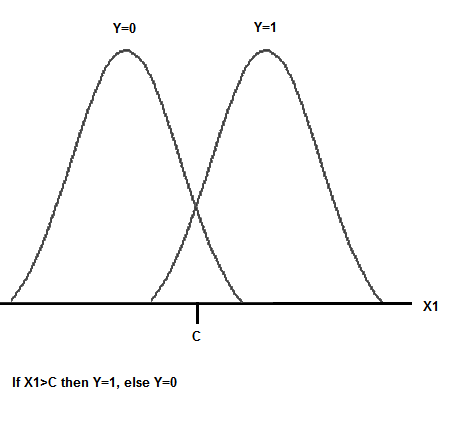
\includegraphics[width=0.5\textwidth]{Gaussians.png}
    \end{figure}
    
    \textbf{Select one:}
    \begin{list}{}
        \item $\circle$ Yes, this can occur if the Gaussians are of equal means and equal variances.
        \item $\circle$ Yes, this can occur if the Gaussians are of equal means and unequal variances.
        \item $\CIRCLE$ Yes, this can occur if the Gaussians are of unequal means and equal variances. 
        \item $\circle$ No, this cannot occur regardless of the relationship of the means or variances.
    \end{list}

    
    
    \clearpage
    
    \item \textbf{[4 pt]} Suppose that $0.3\%$ people have cancer. Someone decided to take a medical test for cancer. The outcome of the test can either be positive (cancer) or negative (no cancer). The test is not perfect - among people who have cancer, the test comes back positive 97\% of the time. Among people who don’t have cancer, the test comes back positive 4\% of the time. For this question, you should assume that the test results are independent of each other, given the true state (cancer or no cancer). What is the probability of a test subject having cancer, given that the subject’s test result is positive?
    
    If your answer is in decimals, answer with precision 4, e.g. (6.051, 0.1230, 1.234e+7)

    \textbf{Fill in the blank:}
    
    \begin{tcolorbox}[fit,height=1cm, width=4cm, blank, borderline={1pt}{-2pt},nobeforeafter]
    
    \begin{center}\huge0.0680\end{center}
    \end{tcolorbox}
    
    
    \item \textbf{[4 pt]} In a Naive Bayes problem, suppose we are trying to compute $P(Y\mid X_1,X_2,X_3,X_4)$ .  Furthermore, suppose  $X_2$  and  $X_3$  are identical (i.e., $X_3$  is just a copy of $X_2$ ).  Which of the following are true in this case?

    \textbf{Select all that apply:}
    \begin{list}{}
        \item $\blacksquare$ Naive Bayes will learn identical parameter values for $P(X_2|Y)$ and $P(X_3|Y)$.
        \item $\square$ Naive Bayes will output probabilities $P(Y|X_1,X_2,X_3,X_4)$ that are closer to 0 and 1 than they would be if we removed the feature corresponding to $X_3$.
        \item $\blacksquare$ This will not raise a problem in the output  $P(Y|X_1,X_2,X_3,X_4)$ because the conditional independence assumption will correctly treat this situation.
        \item $\square$ None of the above
    \end{list}
    
    
    \item \textbf{[3 pt]} Which of the following machine learning algorithms are probabilistic generative models?

    \textbf{Select one:}
    \begin{list}{}
        \item $\circle$ Decision Tree
        \item $\circle$ K-nearest neighbors
        \item $\circle$ Perceptron
        \item $\CIRCLE$ Naive Bayes
        \item $\circle$ Logistic Regression
        \item $\circle$ Feed-forward neural network
    \end{list}
    

\clearpage

\item \textbf{[15 pt]} Logistic Regression and Naive Bayes. 
% \section*{Logistic Regression and Naive Bayes.}

When Y is Boolean and $\Xv = \langle{X_{1}...X_{n}}\rangle$ is a vector of continuous variables, then the assumptions of the Gaussian Naive Bayes classifier imply that $P(Y \mid \Xv)$ is given by the logistic function with
appropriate parameters W. In particular:

\begin{align*}
    P(Y=1\mid\Xv)=\frac{1}{1+\exp(b+\sum_{i=1}^{n} w_iX_i)}
\end{align*}
and
\begin{align*}
    P(Y=0\mid\Xv)=\frac{\exp(b+\sum_{i=1}^{n} w_iX_i)}{1+\exp(b+\sum_{i=1}^{n} w_iX_i)}
\end{align*}

 Consider instead the case where Y is Boolean and ${\Xv = \langle{X_{1}...X_{n}}}\rangle$ is a vector
of Boolean variables. Prove for this case also that $P(Y\mid\Xv)$ follows this same form (and hence that Logistic Regression is also the discriminative
counterpart to a Naive Bayes generative classifier over Boolean features).

\emph{Hints}
\begin{enumerate}
    \item Simple notation will help. Since the $X_{i}$ are Boolean variables, you need only one parameter to define $P(X_{i}\mid{Y} = y_k)$. Define $\phi_{i1} \equiv P(X_{i} = 1\mid{Y = 1})$, in which case $P(X_{i} = 0\mid{Y = 1}) = (1-\phi_{i1}$). Similarly, use $\phi_{i0}$ to denote $P(X_{i} = 1|Y = 0)$.
    \item Notice with the above notation you can represent $P(X_i\mid{Y = 1})$ as follows
\begin{align*}
       P(X_{i}\mid{Y = 1}) = \phi_{i1}^{(X_i)}(1-\phi_{i1})^{(1-X_i)}
\end{align*}
    Note when $X_{i}$ = 1 the second term is equal to 1 because its exponent is zero. Similarly, when $X_{i}$ = 0 the first term is equal to 1 because its exponent is zero.\vspace{1cm}
    
    Write your solution on the following page.
\end{enumerate}
\clearpage
    \begin{tcolorbox}[fit,height=22cm, blank, borderline={1pt}{-2pt},nobeforeafter]
    \begin{equation}\nonumber
    \begin{aligned}
    P(Y = 1\mid\Xv)
    &= \frac{P(\Xv\mid Y = 1)P(Y = 1)}{P(\Xv)}\\
    &= \frac{P(\Xv\mid Y = 1)P(Y = 1)}{P(\Xv\mid Y = 1)P(Y = 1) + P(\Xv\mid Y = 0)P(Y = 0)}\\
    &= \frac{1}{1 + \frac{P(\Xv\mid Y = 0)P(Y = 0)}{P(\Xv\mid Y = 1)P(Y = 1)}}\\
    &= \frac{1}{1 + \exp(\ln\frac{P(\Xv\mid Y = 0)P(Y = 0)}{P(\Xv\mid Y = 1)P(Y = 1)})}\\
    &= \frac{1}{1 + \exp(\ln\frac{P(Y = 0)}{P(Y = 1)} + \sum_{i}\ln\frac{P(X_{i}\mid Y = 0)}{P(X_{i}\mid Y = 1)})}\\
    &= \frac{1}{1 + \exp(\ln\frac{P(Y = 0)}{P(Y = 1)} + \sum_{i}\ln\frac{\phi_{i0}^{(X_i)}(1-\phi_{i0})^{(1-X_i)}}{\phi_{i1}^{(X_i)}(1-\phi_{i1})^{(1-X_i)}})}\\
    &= \frac{1}{1 + \exp(\ln\frac{P(Y = 0)}{P(Y = 1)} + \sum_i(X_i\ln{\frac{\phi_{i0}}{\phi_{i1}}} + (1-X_i)\ln\frac{(1-\phi_{i0})}{(1-\phi_{i1})}))}\\
    &= \frac{1}{1 + \exp(\ln\frac{P(Y = 0)}{P(Y = 1)} + \sum_i\ln{\frac{1-\phi_{i0}}{1-\phi_{i1}}}+ \sum_iX_i(\ln{\frac{\phi_{i0}}{\phi_{i1}}} - \ln\frac{(1-\phi_{i0})}{(1-\phi_{i1})}))}\\
    \end{aligned}
    \end{equation}
    Let $b = \ln\frac{P(Y = 0)}{P(Y = 1)} + \sum_i\ln{\frac{1-\phi_{i0}}{1-\phi_{i1}}}$ and $w_i = \ln{\frac{\phi_{i0}}{\phi_{i1}}} - \ln\frac{(1-\phi_{i0})}{(1-\phi_{i1})}$, then
    \begin{equation}\nonumber
    P(Y=1\mid\Xv)=\frac{1}{1+\exp(b+\sum_{i=1}^{n} w_iX_i)}\\
    \end{equation}
    \begin{equation}\nonumber
    P(Y=0\mid\Xv)=1 - P(Y=1\mid\Xv) = \frac{\exp(b+\sum_{i=1}^{n} w_iX_i)}{1+\exp(b+\sum_{i=1}^{n} w_iX_i)}
    \end{equation}
    \end{tcolorbox}


\end{enumerate}

 \clearpage




\clearpage


\begin{comment} 
{\bf Collaboration Questions} After you have completed all other components of this assignment, report your answers to the collaboration policy questions detailed in the Academic Integrity Policies found \href{http://www.cs.cmu.edu/~mgormley/courses/10601-s18/about.html#7-academic-integrity-policies}{here}.
    \begin{enumerate*}
        \item Did you receive any help whatsoever from anyone in solving this assignment? If so, include full details.
        \item Did you give any help whatsoever to anyone in solving this assignment? If so, include full details?
        \item Did you find or come across code that implements any part of this assignment ? If so, include full details.
    \end{enumerate*}
    
    \begin{tcolorbox}[fit,height=3cm,blank, borderline={1pt}{-2pt},nobeforeafter]
    %Input your solution here.  Do not change any of the specifications of this solution box.
    \end{tcolorbox}
\end{comment}


\textbf{Collaboration Questions} Please answer the following:


    After you have completed all other components of this assignment, report your answers to the collaboration policy questions detailed in the Academic Integrity Policies found \href{http://www.cs.cmu.edu/~mgormley/courses/10601bd-f18/about.html#7-academic-integrity-policies}{here}.
    \begin{enumerate}
        \item Did you receive any help whatsoever from anyone in solving this assignment? Is so, include full details.
        \item Did you give any help whatsoever to anyone in solving this assignment? Is so, include full details.
        \item Did you find or come across code that implements any part of this assignment ? If so, include full details.
    \end{enumerate}
    
    \begin{solution}
    1. No\\
    2. No\\
    3. No
    \end{solution}
    

\end{document}
